
\section{Lecture 30: Simple harmonic oscillations of suspended solid bodies}

The first half (or so) of this lecture is mostly a review of physical pendula. I will make the notes for that part rather brief, as it's easy to go back to previous chapters of these notes for a review.

We will make frequent use of a formula we derived in lecture 21 (and also derived here in lecture very quickly).

\begin{equation}
T = 2 \pi \sqrt{\frac{I_P}{b M g}}
\end{equation}

where $b$ is the distance between the point a pendulum is fixed, and its center of mass. This was derived for a rod, but holds for any geometry, as shown in this lecture. We will use it for rods, hula hoops, solid disks and simple pendula (a mass on a massless string) here. All we need to do is find $b$ and  $I_P$, the moment of inertia about the point where it is fixed (and therefore rotates); when that is done, we can easily calculate the period of that system.

\subsection{Rod}

For a rod, $I_{cm} = (1/12) M \ell^2$. The point P is then located a distance $b = (\ell/2)$ from the center of mass, as we rotate it about its end. Using the parallel axis theorem, $I_P = I_cm + M b^2 = (1/12) M \ell^2 + M \ell^2/4 = (1/3) M \ell^2$. Using those two equivalences,

\begin{equation}
T_{rod} = 2 \pi \sqrt{\frac{(1/3) M \ell^2}{(\ell/2) M g}} =  2 \pi \sqrt{\frac{2 \ell}{3g}}
\end{equation}

The lecture has a demonstration about several pendulum types, where each has a period of approximately 1 second. We want to know how long/large each type of pendulum should be to match that, so let's solve this for $\ell$ also:

\begin{equation}
\frac{3 g T_{rod}^2}{8\pi^2} = \ell
\end{equation}

For $T = \SI{1}{s}$, $\ell \approx 37.27$ cm, assuming we rotate it about the exact end.

\subsection{Simple pendulum}

Next, they ask how long a simple (``regular'') pendulum should be to have a period of 1 second. We use find the period of such a pendulum using the first equation above, using $b = \ell$ and $I_P = M \ell^2$. Doing so quickly gives you

\begin{equation}
T_{simple} = 2 \pi \sqrt{\frac{\ell}{g}}
\end{equation}

Again, let's solve for $\ell$.

\begin{equation}
\frac{g T_{simple}^2}{4 \pi^2} = \ell
\end{equation}

Here, we find a length of about $24.85$ cm.

\subsection{Ring}

We repeat the process for a ring, e.g. a hula hoop, where all the mass can be approximated to be at the circumference. Its center of mass will then be at the geometrical center, i.e. mid-air. Physics doesn't care, and we can use the same formula anyway. Quite amazing, really.\\
Here, we find a moment of inertia of $M R^2$ about the center of mass. Since point P is a distance $b = R$ away, we must add to that $M R^2$ from the parallel axis theorem, and find $I_P = 2 M R^2$.

\begin{equation}
T_{ring} = 2 \pi \sqrt{\frac{2 R}{g}}
\end{equation}

As the professor notes, this is exactly what you would find for a simple pendulum of length $\ell = 2 R$, i.e. with the same length as the diameter of the hula hoop. That makes it a bit unnecessary to solve for $R$, since we could just say that $R = \ell/2$, but I will do so anyway for completeness.

\begin{equation}
\frac{g T_{ring}^2}{8\pi^2} = R
\end{equation}

As expected, we find $R \approx 12.42$ cm, half (ignoring rounding) the length of the simple pendulum. 

\subsection{Solid disk}

Finally, we do this for a solid disk (solid except for a negligibly small hole where it's fixed, of course). Here, $I_{cm} = (1/2) M R^2$, and so adding $M R ^2$ for the parallel axis theorem gives us $(3/2) M R^2$.

\begin{equation}
T_{disk} = 2 \pi \sqrt{\frac{3R}{2g}}
\end{equation}

Or, solved for $R$:

\begin{equation}
\frac{g T_{disk}^2}{6 \pi^2} = R
\end{equation}

$R \approx 16.56$ cm, or $d = 33.12$ cm, which is $4/3$ times that of the hollow ring.\\
The rod must also be exactly 50\% longer than the simple pendulum.

\subsection{Lecture question}

``Suppose we scale up the radius of our planet (keeping its mass density fixed), and the size and mass of a physical pendulum by a factor of 2. How will the period of oscillation change?''

Hmm... Many things will have to change, $g$ being one. Let's first find the change in Earth's mass, and then after that find the change in $g$, before we move on to the pendulum.

Even before that, the period of an ideal pendulum (which I chose from the various types as it's simple) is given by

\begin{equation}
T = 2 \pi \sqrt{\frac{\ell}{g}}
\end{equation}

For a uniform density, we have $M_{old} = (4/3) \rho \pi R^3$ and $M_{new} = (4/3) \rho \pi (2R)^3$, so the mass goes up by a factor of 8 from the $2^3$.\\
The distance to the center of the Earth also doubles, so $g$ changes not only due to the increased mass:

\begin{equation}
\frac{g_{new}}{g_{old}} = \frac{(8 GM)/(2R)^2}{(G M)/R^2} = \frac{8R^2}{(2R)^2} = 2
\end{equation}

So $g$ doubles. Since the period depends on $\ell/g$, which becomes $(2\ell)/(2g)$, the period is unchanged.

\subsection{Oscillating liquid in a U-tube}

Let's now move away from the fairly familiar territory above into something new: oscillating liquids.\\
We have a liquid in a U-shaped tube. The entire mass of the liquid is $M$, the density $\rho$ and the ``length'' of the liquid, at the center of the tube, is $\ell$.

The tube has a cross-sectional area $A$ everywhere along it.

\begin{figure}[H]
\centering
\begin{tikzpicture}[scale=0.5]
\tikzstyle{every node}=[font=\LARGE]
	\draw (3.75,25) -- (3.75,16);
	\draw (4.75,25) -- (4.75,16);
	\draw (11.5,25.25) -- (11.5,16);
	\draw (12.5,25.25) -- (12.5,16);
	\draw (11.5,16) .. controls (10.5,12.5) and (6,12.5) .. (4.75,16);
	\draw (3.75,16) .. controls (5.25,11.25) and (11,11.25) .. (12.5,16);
	\draw (3.75,18) -- (4.75,18);
	\draw (11.5,19.75) -- (12.5,19.75);
	\draw (11.5,22.25) -- (12.5,22.25);
	\draw (3.75,25) .. controls (4,24.75) and (4.5,24.75) .. (4.75,25);
	\draw (11.5,25.25) .. controls (11.75,25) and (12.25,25) .. (12.5,25.25);
	\draw (11.5,25.25) .. controls (11.75,25.5) and (12.25,25.5) .. (12.5,25.25);
	\draw (3.75,25) .. controls (4,25.25) and (4.5,25.25) .. (4.75,25);
	\draw[red] (4.25,18) .. controls (4.25,16) and (3.75,15.75) .. (5.75,13.75);
	\draw[red] (5.75,13.75) .. controls (8,12) and (10,13) .. (11.25,14.5);
	\draw[red] (11.25,14.5) .. controls (12,15.5) and (12.25,15.75) .. (12,17.5);
	\draw[->, >=Stealth, red] (12,17.5) -- (12,19.75);
	\draw[->, >=Stealth, green] (4.5,15.25) -- (5.25,14.25) node[at start, below=8mm] {$v$};
	\draw[->, >=Stealth, green] (7.25,13) .. controls (8,12.75) and (8.25,12.75) .. (9,13) node[midway, below=5mm] {$v$};
	\draw[->, >=Stealth, green] (10.75,14) .. controls (11.25,14.25) and (11.25,14.25) .. (11.5,15) node[right=6mm] {$v=\dot{y}$};
	\draw[->, >=Stealth, green] (11.75,19.5) -- (11.75,21.25) node[at start, right=7mm] {$v$};
	\draw[dashed, red] (12,18.5) -- (13.25,18.5) node[right] {$\ell$};
	\draw[dashed] (12.5,19.75) -- (13.5,19.75);
	\draw[->, >=Stealth] (13.25,19.75) -- (13.25,22.25) node[midway, right] {$y$};
	\draw[->, >=Stealth] (5.25,20) -- (5.25,18);
	\draw (12,25.25) .. controls (12.5,25.75) and (12.5,25.5) .. (13,25.75) node[right] {$A$};
	\draw (4,17.5) -- (4.5,17.75);
	\draw (4,16.75) -- (4.5,17);
	\draw (4,15.75) -- (4.5,16);
	\draw (4.5,15) -- (4.75,15.25);
	\draw (5.25,13.75) -- (5.75,14);
	\draw (6.25,13.25) -- (6.75,13.5);
	\draw (7.75,12.75) -- (8.25,13.25);
	\draw (9.5,13) -- (10,13.75);
	\draw (10.5,13.5) -- (11,14.5);
	\draw (11.75,15.5) -- (12,15.75);
	\draw (11.75,16.75) -- (12.25,17.25);
	\draw (11.75,18) -- (12.25,18.25);
	\draw (11.75,19) -- (12.25,19.25);
	\draw (11.75,20) -- (12.25,20.25);
	\draw (11.75,20.25) -- (12.25,20.5);
	\draw (11.75,20.75) -- (12.25,21);
	\draw (11.75,21) -- (12.25,21.25);
	\draw (11.75,21.5) -- (12.25,21.75);
	\draw (11.75,21.75) -- (12.25,22);
	\node at (17,23) {$M=A\ell\rho$};
	\node at (17,24) {$M\rho A\ell$};
\end{tikzpicture}
\end{figure}

As shown above, we displace the liquid so that it is at a height $y$ above equilibrium height on one side, and a height $y$ below at the other. We also denote the velocity of the liquid as $v = \dot{y}$, which is the same everywhere, at one instant.\\
Say we denote the equilibrium point as $U = 0$ for the system, where $U$ is the gravitational potential energy.\\
If we then displace some liquid as shown, say of mass $\Delta m$, the increase in gravitational potential energy is simply $\Delta m g y$, using $\Delta U = m g h$ with other variable names. This works because the same amount of liquid that is above equilibrium on the right side must be taken from the left side, and so it is equivalent to simply lifting that liquid up a distance $y$, regardless of which side this happens on.

There will be frictional losses and such in this system, but if we neglect that for a while, we can derive an approximate period of oscillation by using the conservation of mechanical energy.

In doing so, we find

\begin{equation}
\frac{1}{2} M (\dot{y}) + \Delta m g y = \text{constant}
\end{equation}

If we substitute in $M = A \ell \rho$ and $\Delta m = A y \rho$,

\begin{equation}
\frac{1}{2} A \ell \rho (\dot{y})^2 + A \rho g y^2 = \text{constant}
\end{equation}

If we take the time derivative, we will have a differential equation in $y$ which has $\ddot{y}$ as the highest derivative. Let's do that and see:

\begin{align}
\frac{1}{2} A \ell \rho 2 (\dot{y}) \ddot{y} + A \rho g 2 y \dot{y} &= 0\\
\ell \ddot{y} +  2 g y &= 0\\
\ddot{y} +  \frac{2 g}{\ell} y &= 0
\end{align}

Many things cancel, including $\dot{y}$. We get a result that is clearly a simple harmonic oscillation! However, more in this case than we have seen previously, this result is not that accurate; at least not for the demonstration in lecture. There is a lot of damping, i.e. the amplitude goes down from its maximum quickly, and as that happens, the period is affected.\\
Anyhow, we know the solution to this differential equation very well by now:

\begin{align}
y &= y_{max} \cos(\omega t + \varphi)\\
\omega &= \sqrt{\frac{2 g}{\ell}}\\
T_{tube} &= 2 \pi \sqrt{\frac{\ell}{2 g}}
\end{align}

This happens to be the same answers as you would find for a simple pendulum of length $\ell/2$ -- nature is funny that way.

Solved for $\ell$, since we did that for the rest,

\begin{equation}
\frac{g T_{tube}^2}{2 \pi^2} = \ell
\end{equation}

For $T = 1$ s, we need $\ell = 0.497$ m or about 50 cm.

\subsection{Torsional pendulum}

Nature really loves these simple harmonic oscillators. Granted, in many of these derivations we use a small angle approximation, but still.\\
For this one, we won't need to do that.

In a torsional pendulum, we can have for example an object hanging from a wire, which we rotate, and then let the wire's restoring torque try to get itself back to equilibrium.\\
Like a simple spring pendulum, a torsional pendulum has a period that is independent of the amplitude, assuming we don't permanently deform the wire, and stay in a region where the restoring torque can be considered linear with regard to the angle we twist the wire.

Consider this system:

\begin{figure}[H]
\centering
\begin{tikzpicture}[scale=0.6]
\tikzstyle{every node}=[font=\LARGE]
	\draw (10,29) -- (10,20.75) node[midway, right] {$\ell$};
	\draw (9.5,29) -- (10.5,29);
	\draw (9.75,29) -- (10,29.25);
	\draw (10.25,29) -- (10.5,29.25);
	\draw (6.5,20.75) -- (13.5,20.75);
	\draw (6.5,20.75) -- (6.5,20.25);
	\draw (13.5,20.75) -- (13.5,20.25);
	\draw (6.5,20.25) -- (13.5,20.25);
	\draw (7.25,20) circle (0.5cm);
	\draw (12.75,20) circle (0.5cm);
	\draw (15.75,24) -- (24.25,24);
	\draw (15.75,24.75) -- (24.25,24.75);
	\draw (15.75,24) -- (15.75,24.75);
	\draw (24.25,24) -- (24.25,24.75);
	\fill (19.75,24.4) circle (3pt) node[below=3mm] {$P$};
	\fill (10,20.5) circle (3pt) node[below=3mm] {$P$};
	\draw[dashed] (16.25,21.75) -- (23.75,27.5);
	\draw (21.25,25.5) .. controls (21.5,25.25) and (21.75,25) .. (21.75,24.75) node[midway, right] {$\theta$};
\end{tikzpicture}
\end{figure}


(Left: as seen from the front; right: as seen from above, after giving the mass a small twist.)

The torque relative to point P is given by

\begin{equation}
\tau_P = -\kappa \theta
\end{equation}

where $\kappa$ (Greek letter kappa) is the \emph{torsional spring constant}. Just as with a spring oscillator, we have a minus sign to denote a restoring torque (or force, in that case), a spring constant, and something the torque/force is proportional to: here an angle, but in the case of a regular spring oscillator, a displacement.

Since the product $\kappa \theta$ must be in newton-meters, and $\theta$ is in radians, the units of $\kappa$ must be N m/rad (though radians are dimensionless, and perhaps we could say the units are already in N m, though that would be a bit confusing).

The torque is always equal to $I_P \alpha = I_P \ddot{\theta}$, so 

\begin{align}
- \kappa \theta &= I_P \ddot{\theta}\\
\ddot{\theta} + \frac{\kappa}{I_P} \theta &= 0
\end{align}

which is a simple harmonic oscillation -- without using any small angle approximation. As usual, the solution to this differential equation is

\begin{align}
\theta    &= \theta_{max} \cos(\omega t + \varphi)\\
\omega &= \sqrt{\frac{\kappa}{I_P}}\\
T          &= 2 \pi \sqrt{\frac{I_P}{\kappa}}
\end{align}

where $\omega$ is the angular frequency, a constant, not to be confused with $\dot{\theta}$ which is the angular velocity. The angular velocity varies with time; it is at a maximum at $\theta = 0$, and zero at $\theta = \theta_{max}$.

$\kappa$ is a function of the cross-sectional area, the length, and of course of the material in question. If the wire is thicker, $\kappa$ will go up, as we would expect; if you instead make it longer, $\kappa$ goes down.\\
Both are intuitive: a thick wire is much harder to turn than a thin one. Also, if you make it longer, it becomes easier to twist -- that also makes sense. A very short steel wire/rod is almost impossible to twist 10 degrees while grabbing each end of the wire/rod, but if it's very long, it's not a problem (unless it's also very thick, so that $\kappa$ is high for that reason).\\
Exactly how this is calculated is not shown, as it is a apparently more complex than the equivalent calculation for the linear case, using Young's modulus.

In the lecture demonstration, we have a 2.5 meter long piano wire, which is either 25/1000" or 1/25000" thick -- the subtitles say the latter, but I'm doubtful. It's a piano wire, which (according to Wikipedia) usually range from about 1/30 to 1/3 inches in diameter. Why would this one be a hundred times thinner?\\
In either case, the professor calculates $\kappa \approx 4 \times 10^{-4}$ Nm/rad for this wire.

If we now calculate the moment of inertia, we can predict the period of the pendulum.\\
We ignore the moment of inertia of the wire, since it's very thin, and has a near-zero moment of inertia about this rotation axis.

Here's a closeup of the part of the system with a non-negligible moment of inertia:

\begin{figure}[H]
\centering
\begin{tikzpicture}[scale=0.6]
\tikzstyle{every node}=[font=\LARGE]
	\draw (3.5,26.75) -- (19.25,26.75);
	\draw (3.5,26.75) -- (3.5,25);
	\draw (3.5,25) -- (19.25,25);
	\draw (19.25,25) -- (19.25,26.75);
	\draw (3.5,25) -- (3.5,23.5);
	\draw (3.5,23.5) -- (5.75,23.5);
	\draw (5.75,23.5) -- (5.75,25);
	\draw (19.25,25) -- (19.25,23.5);
	\draw (19.25,23.5) -- (16.75,23.5);
	\draw (16.75,23.5) -- (16.75,25);
	\draw[dashed] (11,21.5) -- (11,28.75);
	\draw[dashed] (4.5,21.75) -- (4.5,25);
	\draw[dashed] (18,23.5) -- (18,25);
	\draw[<->, >=Stealth, dashed] (4.5,22.25) -- (11,22.25) node[midway, below] {$30$cm};
	\draw[<->, >=Stealth, dashed] (11,24) -- (18,24) node[midway, below] {$30$cm};
	\draw (4.5,24.25) -- (2.5,23.25) node[left] {$0.2$};
	\draw (18,24.25) -- (20.75,24) node[right] {$0.2$kg};;
\end{tikzpicture}
\end{figure}

We can approximate the masses as point particles, each having a moment of inertia of $M R^2$ about the center axis (point P), so the total moment of inertia is approximately $I_P \approx 2 M R^2 = 2(\SI{0.2}{kg})(\SI{0.3}{m})^2 = \SI{0.036}{kg m^2}$.

Using the equation we found earlier, we find $T = \SI{59.608}{s} \approx \SI{60}{s}$.

The rest of the lecture is then demonstrations of this concept. The prediction is fairly accurate even for very large angles -- multiple rotations, not just some 30 degrees or such. The angular velocity is then very high (at times) for large angular displacements, since it must rotate much longer in the amount of time (since the period is independent of amplitude). As mentioned earlier, this is only true as long as we don't leave the region where Hooke's law is valid, and/or permanently deform the wire.

For half a period at 1 rotation, $T = 28.8$ s is measured. For three full rotations, half a period is measured as 28.5 seconds. For 10(!) full rotations, the period is measured as 29.2 seconds.\\
There is a reasonable amount of uncertainty in the measurements, as it's hard to define exactly when it stops rotating. Also, our calculations themselves were really approximations (e.g. the moment of inertia about the rotational axis).

\section{Lecture 31: Pendulums and springs}

We have talked considerably about springs in the past, but we will now add a new twist: instead of just setting a spring system off equilibrium and then leave it be, we apply a time-varying force at some fixed frequency that we choose -- which does not have to be the same frequency that the system would oscillate at on its own.

\begin{figure}[H]
  \centering
\begin{tikzpicture}[scale=1]

  \draw[decorate, decoration={aspect=0.5, segment length=5mm, amplitude=3.5mm, coil}] 
      (0,0) -- (5,0);
  \draw[-{Stealth}, red] (5,1.0) -- (3,1.0) node[midway, above=1mm] {$-kx$};
	\draw[-{Stealth}, red] (5,0) -- (7.5,0) node[above=1mm] {$F_0\cos{(\omega t)}$};
  \fill (5,0) circle (3mm);
  \draw[thick] (0,-1) -- (0,1);
  \draw[dotted] (3,1) -- (3,-1) node[below] {$x=0$};
  \draw[dotted] (5,0) -- (5,-1) node[below] {$x$};
 
\end{tikzpicture}
\caption{}
\end{figure}



An shown, we have a simple system with a mass $m$ connected to a spring. We drive it with some frequency $F_0 \cos (\omega t)$, where $F_0$ is the amplitude of the applied force.\\
We apply Newton's second law to the system, with $a = \ddot{x}$:

\begin{align}
m \ddot{x} &= - k x + F_0 \cos (\omega t)\\
\ddot{x} + \frac{k}{m} x &=  \frac{F_0}{m} \cos (\omega t)
\end{align}

Looks like a simple harmonic oscillator, except that the right-hand side is not zero, which of course changes things considerably.\\
In the beginning, the behavior can be fairly complex; we call this the transient phase, since it is indeed transient: it goes away after a while.\\
After the transient phase, we enter the \emph{steady state}. Here, the driver has ``won'', and the system oscillates at a steady frequency: that of the driver, so $\displaystyle f = \frac{\omega}{2 \pi}$ for the frequency (unless you prefer the angular frequency $\omega$ as-is). The mass will then move as described by $x = A \cos (\omega t)$, once the transient phase is over. The amplitude $A$ of this oscillation is not known, so let's try to find it.

The derivatives of this trial solution are (since we need $\ddot{x}$):

\begin{align}
x            &= A \cos (\omega t)\\
\dot{x}   &= -A \omega \sin(\omega t)\\
\ddot{x} &= -A \omega^2 \cos(\omega t)
\end{align}

We can then try to substitute $x$ and $\ddot{x}$ above into the differential equation we found earlier.

\begin{align}
-A \omega^2 \cos(\omega t) + \frac{k}{m} A \cos (\omega t) &=  \frac{F_0}{m} \cos (\omega t)\\
A\left(\frac{k}{m} - \omega^2\right)  &=  \frac{F_0}{m}\\
A\left(\omega_0^2 - \omega^2\right)  &=  \frac{F_0}{m}\\
A &=  \frac{F_0}{m\left(\omega_0^2 - \omega^2\right)}
\end{align}

Here, we have used $\displaystyle \omega_0 = \sqrt{\frac{k}{m}}$, which we call the natural frequency of the system. It is the $\omega$ we have seen before in spring systems -- the one it oscillates with naturally, if you offset it from equilibrium and then let it be. We add a subscript 0 to denote this, since $\omega$ is now the driving frequency.

Let's look at some limiting cases. In the case $\omega \ll \omega_0$; in that case, we find $A = F_0/k$.\\
If $\omega \gg \omega_0$, the amplitude goes to 0. (That it also becomes negative is something we will discuss shortly.)

If $\omega \to \omega_0$, i.e. we drive it at the natural frequency, the denominator goes to zero, and the amplitude goes to infinity. It doesn't go to infinity it practice, of course, but the amplitude does tend to become very large. We call this \emph{resonance}.\\
Frictional forces etc. limit the actual amplitude in practice.

If we plot the amplitude $A$ versus the driving (angular) frequency $\omega$, we find something like this:

\begin{figure}[H]
  \centering
\begin{tikzpicture}
	\begin{axis}[axis lines=middle,samples=200,ticks=none,xlabel={$\omega$},ylabel={$A$}]
		\addplot[domain=-0.4:1.85] {1/(2-x)};
\addplot[domain=2.15:6] {1/(2-x)};
		\draw[dashed] (axis cs:2,-8) -- (axis cs:2,10) node[midway, left] {$\omega_0$};
\end{axis}
	\node at (-0.3, 3.1) {$\frac{F_0}{k}$};
	\node at (0, 2.6) {$0$};
\end{tikzpicture}
\end{figure}


The negative values mean that the object is now 180 degrees out of phase with the driver, which we don't go into any detail about in this lecture.

If we take a more realistic case (where the amplitude stays finite), and also plot the absolute value of the amplitude to get rid of the discontinuity of the phase shift, we get something like this:

\begin{figure}[H]
  \centering
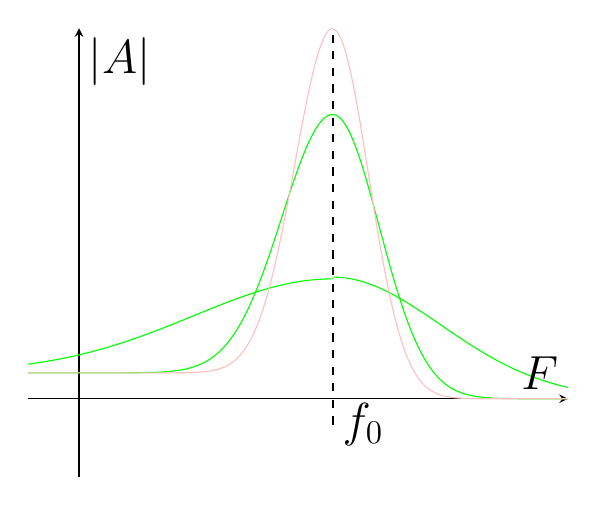
\begin{tikzpicture}
\begin{axis}[axis lines=middle, ymin=-0.3,samples=200,ticks=none,xlabel={$F$},ylabel={$|A|$}]
	\addplot[green,domain=-0.4:2.0] {0.1+1/(1.1*sqrt(2*pi)*e^((1/2)*((x-2)/1.1)^2))};
	\addplot[green,domain=2.0:3.85] {1/(0.85*sqrt(2*pi)*e^((1/2)*((x-2)/0.85)^2))};
	\addplot[green,domain=-0.4:2.0] {0.1+1/(0.4*sqrt(2*pi)*e^((1/2)*((x-2)/0.4)^2))};
	\addplot[green,domain=2.0:3.85] {1/(0.364*sqrt(2*pi)*e^((1/2)*((x-2)/0.364)^2))};
	\addplot[pink,domain=-0.4:2.0] {0.1+1/(0.3*sqrt(2*pi)*e^((1/2)*((x-2)/0.3)^2))};
	\addplot[pink,domain=2.0:3.85] {1/(0.28*sqrt(2*pi)*e^((1/2)*((x-2)/0.28)^2))};
\draw[dashed] (axis cs:2,-0.1) -- (axis cs:2,10) node[at start, right] {$f_0$};
\end{axis}
\end{tikzpicture}
\end{figure}


The less damping there is, the narrower the resonance peak is (shown in pink). With lots of damping, the peak becomes just a small bump (in green).

If we have a more complex system with more than 1 mass, all joined together with springs, we find the same number of resonance frequencies as there are masses, so a plot of amplitude vs driving frequency would have multiple peaks.\\
We can take this to the extreme, and consider a practically infinite number of such oscillators, in for example a violin string. We can think of each atom being a mass, connected to the others via a ``spring'' (in reality via electromagnetic forces).

In the case we have looked at earlier, we have a case of longitudinal oscillations: the objects move in the same direction as the spring, so to speak.\\
Oscillations/waves can also be transverse; electromagnetic waves are transverse, for example. Water waves are not good as an example, as they are a combination; in a fully transverse water wave, each molecule of water would simply move up and down, as the wave passes from side to side.

Sound is a longitudinal wave; at least in air, there appears to be some discussion about whether transverse waves in other media can be considered sound or not.

\subsection{Harmonics}

Let's look now at the example of shaking a string. As mentioned earlier, there will be many, many resonance frequencies. Consider the first few:

\begin{figure}[H]
  \centering
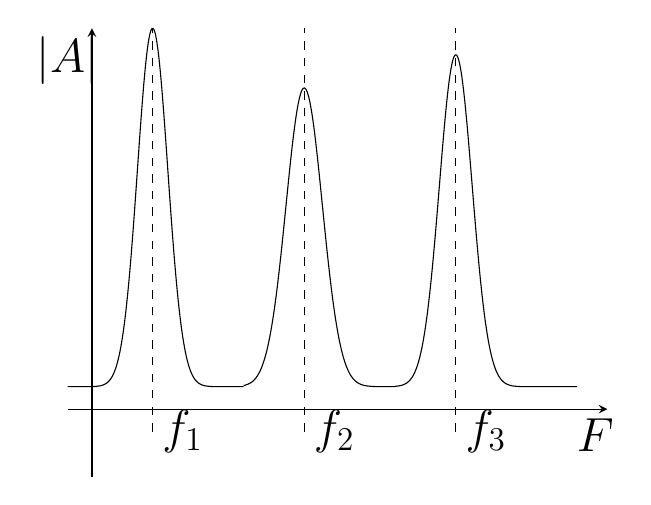
\begin{tikzpicture}
	\begin{axis}[axis lines=middle,ymin=-0.3,xmax=8.5,samples=200,ticks=none,x label style={at={(axis cs:8.3,-0.0)},anchor=north},xlabel={$F$},y label style={at={(axis cs:-0.4,1.7)},anchor=north},ylabel={$|A|$}]
	\addplot[domain=-0.4:2.5] {0.1+1/(0.25*sqrt(2*pi)*e^((1/2)*((x-1)/0.25)^2))};
	\addplot[domain=2.5:5.0] {0.1+1/(0.3*sqrt(2*pi)*e^((1/2)*((x-3.5)/0.3)^2))};
	\addplot[domain=5.0:8.0] {0.1+1/(0.27*sqrt(2*pi)*e^((1/2)*((x-6)/0.27)^2))};
\draw[dashed] (axis cs:1,-0.1) -- (axis cs:1,10) node[at start, right] {$f_1$};
\draw[dashed] (axis cs:3.5,-0.1) -- (axis cs:3.5,10) node[at start, right] {$f_2$};
\draw[dashed] (axis cs:6,-0.1) -- (axis cs:6,10) node[at start, right] {$f_3$};
\end{axis}
\end{tikzpicture}
\end{figure}


We start off by shaking the string up and down at a low frequency, which we slowly increase. At one point, we will hit the first resonance frequency, also known as the first harmonic, or the fundamental. We denote this frequency as $f_1$.\\
At that point, the amplitude will be much greater than it was just before, and we will have a \emph{standing wave}. Each point of the curve will bob up and down, but that is all that happens. The movement is the greatest at the center, and zero at the two ends where the string is held.\\
Points where the string is standing still are called \emph{nodes} (while points of maximum amplitude are called \emph{antinodes}).

If we keep increasing the frequency, we will eventually find the second resonance frequency, or second harmonic, $f_2$. There will now be a node at the center of the string, while there will be two antinodes, evenly spaced. The two antinodes will be 180 degrees out of phase, so when one is at its highest point, the other is at its lowest.

Increase the frequency further, we find the third harmonic, $f_3$. This adds another node, so there are now two nodes and three antinodes.\\
Animated graphics are extremely useful here, so I suggest looking some up. Wikipedia has one on the page ``Node (physics)'' and several more in the article ``Vibrating string'', which shows the first five harmonics.

Here is a still image from the lecture, which is about the best I can do in these notes (in the lecture, Prof. Lewin also did a demonstration):

\begin{figure}[H]
  \centering
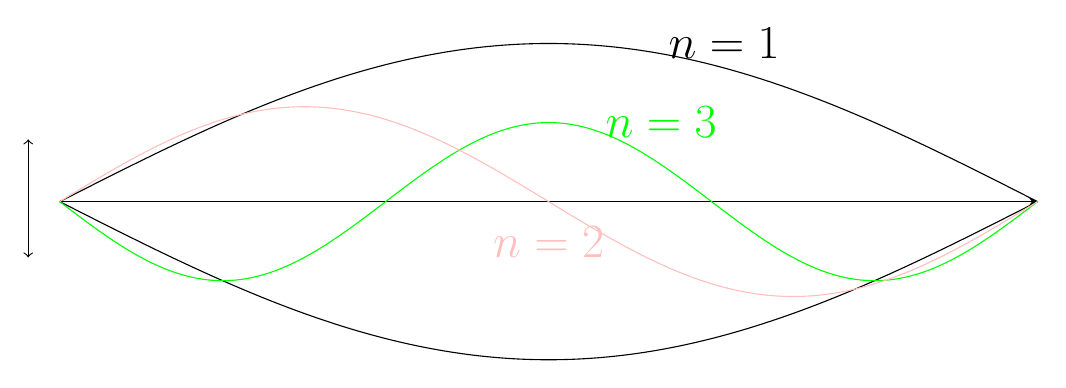
\begin{tikzpicture}
	\begin{axis}[height=6cm, width=14cm, ticks=none, axis y line=none, axis x line=center, xmin=0, xmax=2*pi, ymin=-1.1, ymax=1.1]
		\addplot[domain=0:2*pi, samples=200] { sin(0.5*deg(x)) } node[midway, right=14mm] {$n=1$};
	\addplot[domain=0:2*pi, samples=200] { -sin(0.5*deg(x)) };
	\addplot[green, domain=0:2*pi, samples=200] { -0.5*sin(1.5*deg(x)) } node[midway, right=6mm] {$n=3$};
	\addplot[pink, domain=0:2*pi, samples=200] { 0.6*sin(deg(x)) } node[midway, below=2mm] {$n=2$};
\end{axis}
	\draw[<->] (-0.4,1.5) -- (-0.4,3);
\end{tikzpicture}
\end{figure}


The first harmonic, $n=1$ (in white) just has the string being either all high, all low, or in transition between the two states.\\
The second harmonic, $n=2$ (in pink) has a node at the center, with the antinodes out of phase.\\
The third harmonic, $n=3$ (in green) has two nodes, with the leftmost and rightmost antinodes in phase with each other, and out of phase with the middle antinode.

These frequencies follow a simple relationship of $f_n = n f_1$, i.e. they are integer multiples of the fundamental frequency. If $f_1 = 100$ Hz, then $f_2 = 200 Hz$, $f_3 = 300 Hz$ etc.\\
In musical instruments, the second harmonic is therefore one octave higher than the first. The third harmonic is not one octave higher than the second harmonic, though, but rather an interval of a perfect fifth above.\footnote{In just intonation, a perfect fifth has a frequency ratio of 3:2, i.e. 1.5 times; in equal temperament, which most instruments use in modern times, a perfect fifth is exactly $2^{7/12} \approx 1.4983$ times the frequency of a given note, but this is now really becoming music theory.}  (An octave doubles the frequency, which would be 400 Hz, so the fourth harmonic in an octave above the second.)

The frequency of the fundamental/first harmonic depends on the string's mass, length and tension (or, if you prefer, the mass per unit length, length and tension).

Many musical instruments are of course stringed instruments. In the case of a piano, the strings vary in all three attributes.\\
In a violin, there are four strings, of essentially equal length. The thickness (and therefore mass per unit length) varies. Tuning is set by adjusting the tension in each string individually.\\
A higher tension causes a higher pitch, while a \emph{shorter} string causes a higher pitch (for a given tension and mass).\\
When playing a violin, the player changes the pitch by shortening the strings. When you fret a note (i.e. hold a string down against the violin's neck), the effective length that vibrates is shortened, and so the pitch goes up.

In the case we looked at earlier, with the driven spring and the long shaken string, the driver alone decided the frequency. How does that work in the case of e.g. a violin?\\
When we use a bow on a violin, that rubbing motion can be thought to consist of many, many different frequencies at which the string is ``driven''. The string picks out its resonance frequencies, and so the frequencies we hear are mostly the different harmonics, i.e. integer multiples of the string's fundamental frequency.

The ratio of the amplitudes of the different harmonics is what gives an instrument its \emph{timbre}. Consider a theoretical violin string that only oscillated at a single frequency $f_1$. The sound it would make is a pure sine wave -- which sounds like a very boring ``beep'' and nothing at all like a violin.\\
For a middle A note, both a violin and a piano produce a 440 Hz sound with several harmonics, but they sound very different, as the harmonic content of the two are very different.\\
Adding up only the odd harmonics -- 1, 3, 5 etc -- will produce a square wave, which adding up all harmonics gives a sawtooth wave. These terms are mostly used in synthesis of sound, but are also useful for describing the sound of real-world instruments. Violins have a lot of harmonic content, and are much closer to a sawtooth-shaped waveform than to a square-shaped one in timbre.

\subsection{Woodwind instruments}

Consider an overly simple woodwind instrument: a closed box of length $L$, filled with air, and a loudspeaker at the end that can generate different frequencies. We can find several such resonant frequencies, however, this time it's not the material itself that resonates, but rather the air inside it.\\
The air acts a bit like a spring if you excite it at the right frequencies. The harmonics are easily calculated as

\begin{equation}
f_n = \frac{n v}{2 L}
\end{equation}
where $n$ is the harmonic number, $v$ is the speed of sound in air (about 340 m/s) and $L$ is the length of the box.

This instrument isn't very practical though; it's not only closed, so that the sound will barely be audible outside, but it is driven by a loudspeaker. We can take care of that by opening up either one side, or both. What is now interesting (and rather strange, in my opinion) is that if we open up both sides of this box, and again put the loudspeaker at one end, we can still find the exact same resonance frequencies as we did before!\\
This would be referred to as an open-open instrument. Flutes are open-open (more or less).
We can also open up only one side, to create a closed-open instrument, such as a clarinet. In this case, the formula above doesn't apply; there is no additional detail to how or why it is different, though.

In reality, the loudspeaker is of course replaced by the player (or the player's mouth, rather).

\subsection{Other resonances}

Next, there is some talk about how everything has a resonance frequency: from car keys to frying pans and refrigerators, people and wine glasses.\\
The wine glass is demonstrated: by moving a clean, wet finger around the top of a wine glass, you can generate a fairly loud sound. What happens is just as with the violin string, our rubbing causes a ton of different frequencies to be generated, and the glass ``picks out'' its resonance frequency/frequencies and hums along at those.

Resonances can also be destructive. By playing back a tone that corresponds to the glass' fundamental resonance frequency at a loud volume, we can make the amplitude of oscillation so great that the glass breaks. This is demonstrated using a strobe light setup to allow us to see the deformations in the glass (which are about 470 Hz, which of course is far too fast to see otherwise).

Another well-known and oft-cited example is the Tacoma Narrows Bridge, first opened on July 1, 1940. It collapsed barely more than 4 months later, on a day of strong wind. However, while this is often presented as a resonance phenomena, it appears opinion has changed, and it is now consider to be due to aerodynamic flutter rather than forced oscillation. This is the same phenomena that causes a paper to oscillate when held steadily in constant airflow. Some also present it as a combination of multiple phenomena, and I certainly don't have the expertise to say who is correct, so I'll leave it at that.

Finally, the professor demonstrates what happens when the speed of sound in a medium changes -- or when the medium itself changes, rather, by filling his lungs with helium while speaking. Sound travels about 2.7 times faster in helium than in air, and so the pitch created by our vocal chords goes way up if your lungs are filled with helium rather than air.\\
Since helium is, well, helium, which doesn't contain the $\approx 20$\% oxygen we need to live, this experiment is dangerous if done incorrectly (or for anything but a short period of time).

\section{Lecture 32: Thermal expansion}

We begin the lecture by introducing the concept of thermometric properties. A thermometric property is a property of an object that depends on the object's temperature. A typical one, that we will look at in this lecture, is that many objects expand when heated, and contract when cooled.\\
If we heat up a gas in a closed container, the pressure in the container goes up, which is a thermometric property. If we heat an electric conductor, the electric resistance will tend to go up.\\
(That is why regular light bulbs often break when turned on; the current through them is at a maximum the first split second before it starts to reach its operating temperature (which happens extremely quickly). After that, the resistance goes up, and so the current goes down, to its steady state level.)

If we heat a metal bar, it will expand. Cool it, and it will shrink. If we bring a hot and a cold iron bar together, there will be heat transfer between the objects until they are in thermal equilibrium, i.e. when their temperatures are equal. Until then, the two bars will both change in size as their temperature changes.

We can construct a simple thermometer this way. We have a bar of some length $L$ of a known material, at a known temperature. We put the bar in melting ice, and measure a length $L_1$; we then put it in boiling water, and find a length $L_2$. We can then define a temperature scale such that, for example, $L_1$ means the temperature is 0 degrees, and $L_2$ means 100 degrees. This is basically how the Celsius scale works.\\
This scale is (or was) often called \emph{centigrade} (from Latin's centum, meaning hundred and gradus meaning step), though that name was formally obsoleted in 1948, and the scale is now known as the Celsius scale, after Anders Celsius, the Swedish astronomer who came up with it.\footnote{Apparently, his original scale was the opposite: ice melted at 100 degrees, while water boiled at 0. Carl von Linn\'e, also know as Carl Linnaeus, reversed the scale soon after Celsius' death.}

Another common temperature scale is the Fahrenheit scale, invented by German scientist Daniel Gabriel Fahrenheit. He used brine, a mixture of salt and ice, as the zero degree definition, and human body temperature as 100... roughly speaking, as 98.6 F is the most commonly quoted number for human body temperature these days, and 100 F is defined as having a fever.

Conversion between the two scale is relatively straightforward. 0 degrees C is 32 degrees F, while 100 degrees C is 212 degrees F. To convert, we use

\begin{align}
T_F &= \frac{9}{5} T_C + 32\\
T_C &= \frac{5}{9} \left(T_F - 32\right)
\end{align}

The two scales ``cross over'' at -40 degrees, so $\SI{-40}{{}^\circ\text{F}} = \SI{-40}{\degreeCelsius}$.

The third temperature scale (or perhaps rather unit) that is fairly common, especially very common in science, is the kelvin, which is an absolute temperature scale. Because it is absolute (see below), we do not talk about ``degrees'' kelvin, but just kelvin (just as we don't talk about degrees pascal).
The coldest temperature with any physical meaning, absolute zero, is by definition 0 K. At this temperature, it is often said that all motion stops (which is not entirely true, due to to the world of quantum mechanics), and so colder temperatures are not very meaningful. This might be expanded upon as early as next week, when Heisenberg's uncertainty principle is introduced.

The kelvin scale is closely related to the Celsius scale: it is offset by exactly 273.15 degrees C, so that 0 K = $\SI{-273.15}{\degreeCelsius}$. Therefore, water boils at 373.15 K (at 1 atm of pressure).

\subsection{Thermal expansion}

We can now get to the focus of this lecture: thermal expansion.\\
Say we start with a rod of length $L$. We heat it up by $\Delta T$ degrees C (or kelvin), and it gets longer by an amount $\Delta L$. We can approximate this amount in a simple way:

\begin{equation}
\Delta L = \alpha L \Delta T
\end{equation}

where $\alpha$ is known as the \emph{linear expansion coefficient}, with units of 1 over degrees Celsius ($1/{}^\circ$C).

As the values of $\alpha$ are often small, we can write them in terms of $10^{-6}/{}^\circ$C, equivalent to $\text{ppm/}^\circ$C or ppm/K.\\
$\alpha$ for a few common materials is

\begin{center}
\begin{tabular}{|r|l|}
\hline
$\alpha$ & ppm/${}^\circ$C\\ \hline
Copper & 17\\\
Brass & 19\\
Pyrex & 3.3\\
Invar & 0.9\\
Steel & 12\\
\hline
\end{tabular}
\end{center}

Invar is an alloy often used for its unusually low thermal expansion coefficient. There are several variations; the one usually called invar is 64\% iron and 36\% nickel. It was invented by Swiss scientist Charles \'{E}douard Guillaume in 1896; the invention won him the Nobel prize in physics in 1920.\\
Having a material with a low thermal expansion coefficient is important for many precision instruments, for example.

Consider a steel railroad track, 1000 meters long. In many climates, it might need to be usable at -15 degrees C, a cold winter's day, and also at +35, a hot summer's day, so $\Delta T = 50$ degrees. Using the formula above, and the value of $\alpha$ of steel, we find $\Delta L = 0.6$ meters. If the rail is continuous and can't expand in the ``forward'' direction, it will start to bulge either sideways or upwards, whichever is easier.

How is this taken care of? The rail needs to be able to expand, or it will deform and become unusable. One solution is very simple: the railroad has gaps in it. We need gaps of up to 60 cm per km, so for example 5 cm per 80 meters gives the rail space to expand. With large enough wheels, this causes a ``clunk'' when riding over it, but nothing more.

The professor then demonstrates the expansion of a brass bar, by using an ``amplifier'' device to turn the small (millimeter-scale) expansion into something more clearly visible (a large change in the angle of an indicator).

\subsection{Bimetals}

Bimetals are a very useful type of material. We take two metals with different linear expansion coefficients, and put them together (perhaps using welding):

\begin{figure}[H]
  \centering
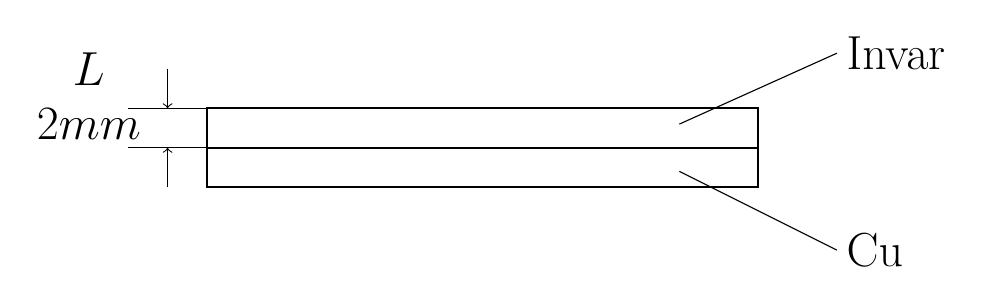
\begin{tikzpicture}
	\draw[thick] (0,0) rectangle (7,0.5);
	\draw[thick] (0,0.5) rectangle (7,1);
	\draw (0,0.5) -- (-1,0.5);
	\draw (0,1) -- (-1,1);
	\draw[->] (-0.5,0) -- (-0.5,0.5);
	\draw[->] (-0.5,1.5) -- (-0.5,1);
	\node at (-1.5,1.5) {$L$};
	\node at (-1.5,0.8) {$2mm$};
	\draw (6,0.8) -- (8,1.7) node[right] {Invar};
	\draw (6,0.2) -- (8,-0.8) node[right] {Cu};
\end{tikzpicture}
\end{figure}



When we heat this system, what happens? The copper must get longer, but the change in the invar's length is much less. Since we join them such that one can not expand without affecting the other, it will bend upwards, so that the invar is on the inside of an arc, and the copper is along the (longer!) outside. The difference in the length change of the two materials is

\begin{equation}
\Delta L_{Cu} - \Delta L_{invar} = (\alpha_{Cu} - \alpha_{invar}) L \Delta T
\end{equation}

For a 10 cm rod composed of copper and invar, the difference in expanded length is about 0.16 mm. However, the difference in height between the two sides will be about 3-4 mm\footnote{The professor says about 4 mm; a scientific paper on bimetal thermostats has a formula that gives about 3 mm; one or both are probably estimates, though.}, despite the small difference in length.

We can use bimetals for example in thermostats, so that a bimetal being sufficiently cold makes contact in an electric circuit, to turn a heater on. Once the bimetal is warm enough, it expands and ``bends away'', so that the contact is broken, and the heater turns off.

They can also be used for safety devices. Gas stoves sometimes use a ``pilot light'', basically a small flame, that is used to light the main burners. If the pilot light is off, but the gas is on, the room will fill up with a flammable and explosive gas, which can of course cause horrible accidents. One of several ways to prevent this is to use a bimetal, such that the gas supply is only on as long as the pilot light is burning. When it goes out, the bimetal cools down, and in some way automatically turns off the gas supply.

We can build thermometers of bimetals. We could have a construction like this:

\begin{figure}[H]
  \centering
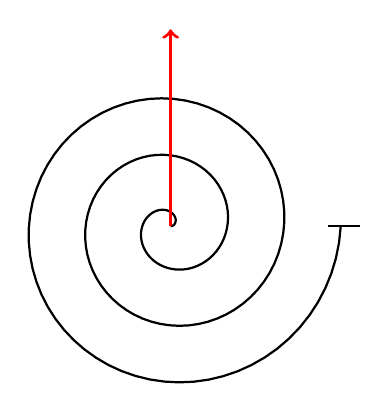
\begin{tikzpicture}[scale=1]

% Spiral
\draw[thick, domain=0:6*pi, variable=\t, samples=200]
  plot ({(\t r)*cos(\t r)/500}, {(\t r)*sin(\t r)/500});

% Central arrow (outward)
\draw[very thick, red, ->] (0,0) -- (0,2.5);

% Little handle-like bar
\draw[thick] (2.0,0) -- ++(0.4,0);

\end{tikzpicture}
\end{figure}

The outer end is attached to some casing and cannot move. The pink arrow is some form of indicator, attached at the center.\\
When the bimetal is heated, it will try to curl up even tighter than it already is, and the arrow moves clockwise. When the bimetal is cooled, the arrow moves towards the left. All we need, then, is to calculate how much it will turn, and then add a temperature scale around this.

Here is such a thermometer:

\begin{center}
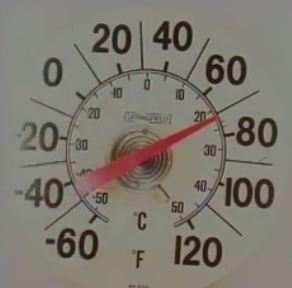
\includegraphics[scale=0.8]{\pIImages/lec32_bimetal_thermometer2}
\end{center}

\subsection{Volumetric expansion}

Let's now consider how much the \emph{volume} of an object increases when heated.\\
For simplicity, we use a cube, of side $L$. We increase the temperature by $\Delta T$.

The old volume is $V = L^3$, and the new volume $V + \Delta V = \left(L + \Delta L\right)^3$. Let's try to approximate this for a small increase in $L$.

\begin{align}
\Delta V &= \left(L + \Delta L\right)^3 - V\\
\Delta V &= L^3 \left(1 +  \frac{\Delta L}{L}\right)^3 - L^3
\end{align}

Here, we simply factor out $L^3$, and then also substitute $V = L^3$.\\
Next, we use the first-order term of the Taylor expansion of $(1 + x)^n \approx 1 + n x$, where $x = \Delta L/L$ and $n = 3$:

\begin{align}
\Delta V &= L^3 (1 + 3 \frac{\Delta L}{L})     - L^3\\
\Delta V &= 3 \frac{L^3 \Delta L}{L}\\
\Delta V &= 3 L^2 (L \alpha \Delta T) \label{eq:lec32eq3}\\
\Delta V &= 3 \alpha L^3  \Delta T\\
\Delta V &= 3 \alpha V  \Delta T
\end{align}

In \eqref{eq:lec32eq3} we simply substitute $\Delta L = L \alpha \Delta T$.\\
We find, then, that the result depends on some value $3 \alpha$. We usually write this as $\beta = 3 \alpha$, and call it the \emph{cubic expansion coefficient} (or volumetric expansion coefficient).

The reason we can use the linear term only is that the next term in the Taylor series contains $\alpha^2$, which is extremely small. (For $L = 1$ m, $\Delta T = 100$ K and $\alpha = 10^{-5}/{}^\circ$C, the quadratic term is $3 \times 10^{-6}$, versus $1.003$ for the two terms we do have. )The higher-order terms are much smaller yet.

We can now look at how a(nother) simple thermometer can work, e.g. a mercury thermometer, though other fluids are used these days, for safety reasons.\\
Mercury has a $\beta$ of about $18 \times 10^{-5}/{}^\circ$C, while Pyrex has a value of roughly $\num{1e-5}$ (3 times the value of $\alpha$ we had earlier). A Pyrex container with mercury inside will then barely expand when heated, but the mercury inside certainly will -- about 18 times as much. If we make a reservoir of mercury at the bottom, and then a very narrow column upwards, we get this:

\begin{figure}[H]
  \centering
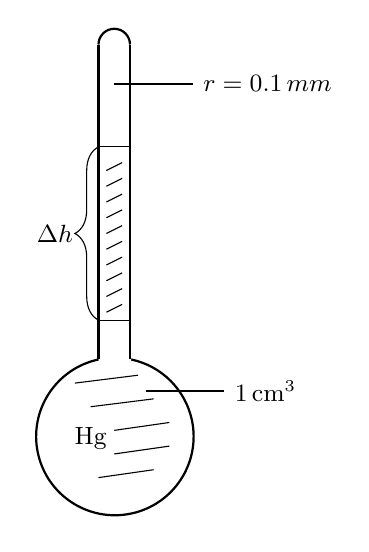
\begin{tikzpicture}

	% Bulb
  \draw[thick] (0,0) arc[start angle=102, end angle=438, radius=1];
	%\draw[thick] (0,0) circle (1);
	
	% Mercury label
	\node at (-0.1,-1) {\small Hg};
	\draw[thick] (0.6,-0.4) -- ++(1,0) node[right] {\small 1\,cm$^3$};
	
	% Capillary tube
	\draw[thick] (0,0) -- (0,4);
	\draw[thick] (0.4,0) -- (0.4,4);
	
	% Top opening
	\draw[thick] (0,4) arc[start angle=180,end angle=0,radius=0.2];
	
	% Shaded height (Δh)
	\draw[decorate, decoration={brace, mirror, amplitude=3mm}] (0,2.7)-- (0,0.5) node[midway, left=2mm] {\small $\Delta h$};
	\draw (0,2.7) -- ++(0.4,0);
	\draw (0,0.5) -- ++(0.4,0);

	\draw (0.1,0.6) -- ++(0.2,0.1);
	\draw (0.1,0.8) -- ++(0.2,0.1);
	\draw (0.1,1.0) -- ++(0.2,0.1);
	\draw (0.1,1.2) -- ++(0.2,0.1);
	\draw (0.1,1.4) -- ++(0.2,0.1);
	\draw (0.1,1.6) -- ++(0.2,0.1);
	\draw (0.1,1.8) -- ++(0.2,0.1);
	\draw (0.1,2.0) -- ++(0.2,0.1);
	\draw (0.1,2.2) -- ++(0.2,0.1);
	\draw (0.1,2.4) -- ++(0.2,0.1);

	\draw (-0.3,-0.3) -- ++(0.8,0.1);
	\draw (-0.1,-0.6) -- ++(0.8,0.1);
	\draw (0.2,-0.9) -- ++(0.7,0.1);
	\draw (0.2,-1.2) -- ++(0.7,0.1);
	\draw (0.0,-1.5) -- ++(0.7,0.1);
	
	% Radius label
	\draw[thick] (0.2,3.5) -- ++(1,0) node[right] {\small $r = 0.1\,\text{mm}$};
	
\end{tikzpicture}
\end{figure}

When the mercury/liquid expands, it has nowhere to go except up the display tube. We calculate how much the column will grow per degree, and create the scale accordingly. All that remains is then to fill it up to the correct level, and nature takes care of the rest.

Consider a tiny radius of 0.1 mm, as shown, for the display tube. Ignoring the expansion of the Pyrex (which we probably shouldn't do if we actually built this), if our 1 cubic centimeter of mercury/liquid goes up in temperature by 10 degrees C, it expands by $V \beta \Delta T = \SI{0.0018}{cm^3}$.\\
A very small increase, but hold on. A height $h$ in the tube can hold a volume $\pi r^2 h$, so we find $\displaystyle h = \frac{\SI{0.0018}{cm^3}}{\pi (\SI{0.01}{cm})^2} = 5.73$ cm! That gives us almost 6 mm per degree, which is quite a bit more than most such thermometers I've seen; very easily readable.

\subsection{Expansion of water}

Water is a peculiar substance. We have so far only talked about substances that expand when heated, but water behaves rather differently at some temperatures.\\
If we take room-temperature water and cool it down slightly, it shrinks, as expected. However, once we reach 4 degrees C, cooling it \emph{further} down to 0 will cause the water to expand!\\
Put in other words, the density of water is at a \emph{maximum} when it is at 4 degrees C. This also implies that in this region between 0 and 4 degrees C, $\beta < 0$, so it changes sign at 4 degrees C.

This causes several important phenomena. For one, the 4 degree water sinks to the bottom, while ice tends to float; therefore, the bottom of lakes and such tend to remain liquid all year round, so that fish can survive below the ice.

For most materials, the solid of a material tends to sink in its liquid (i.e. the solid tends to have a higher density, so that a given amount, measured by mass, is more compact), but water is an exception.

%%% Local Variables:
%%% TeX-master: "../../main"
%%% End:
